\chapter{Metodologia}

% \section{Tipo de Pesquisa}
Uma pesquisa científica pode ser classificada quanto à sua abordagem, sua natureza, seus objetivos e seus procedimentos \cite{gerhardt2009tiposdepesquisa}, dessa forma podemos definir que esta pesquisa terá uma abordagem quantitativa, natureza aplicada, objetivo exploratório, e os procedimentos serão de uma pesquisa exploratória.

Esta seção apresenta a metodologia que será empregada no desenvolvimento do trabalho proposto, visando alcançar os objetivos descritos anteriormente.

% \section{Materiais e Métodos}

\section{Rede de Sensores sem Fio}
A rede de sensores proposta coleta dados de temperatura, umidade do ar e molhamento foliar, com o objetivo de, a partir dos dados coletados, efetuar o controle do sistema nebulizador.

Cada nó da rede é composto por um controlador, neste trabalho foi utilizado a plataforma NodeMCU. Este controlador esta conectado aos sensores DHT11 (responsável pela coleta de temperatura e umidade) e o sensor de molhamento foliar. Todos os nós estão conectados à internet por meio de uma rede \textit{wifi}. A figura \ref{fig:esquema-rede} representa, de forma simples, como é a estrutura da rede.

\begin{figure}[H]
\centering
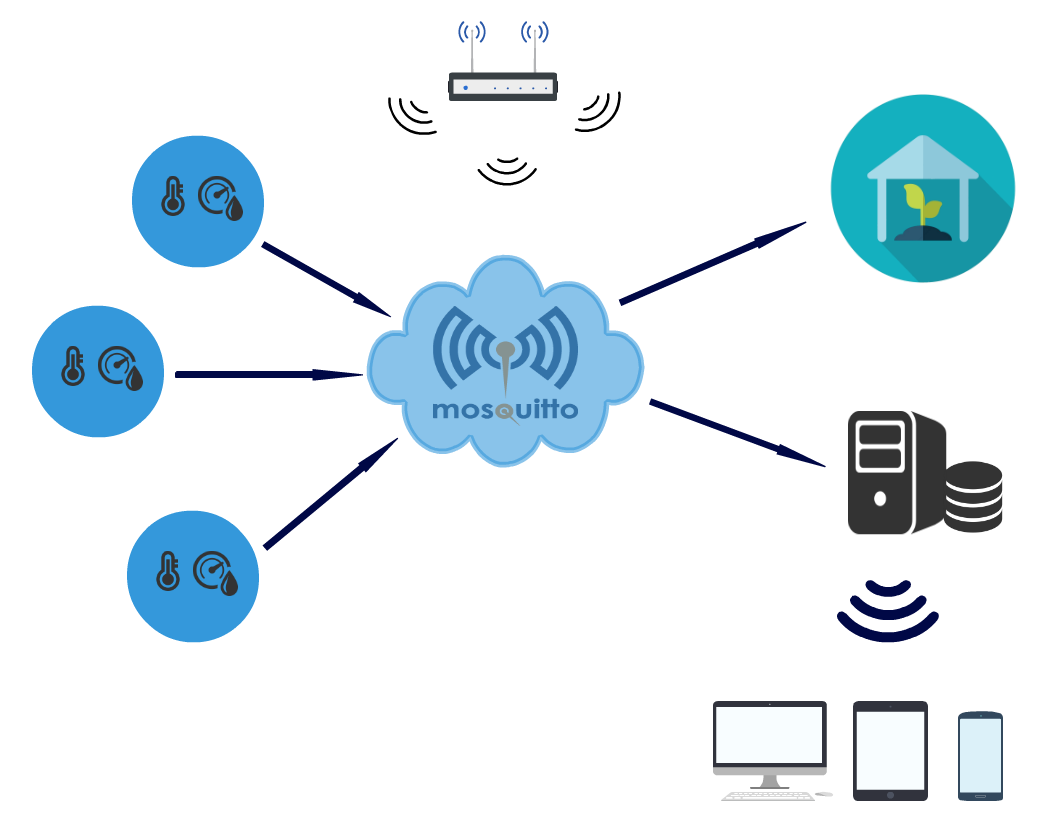
\includegraphics[scale=0.3]{./04-figuras/rede.png}
\caption{Esquema da rede de sensores}
\vspace{-\baselineskip}
\fonte{Do autor}
\label{fig:esquema-rede}
\end{figure}

A comunicação da rede se dá por meio do protocolo MQTT utilizando a ferramenta Mosquitto, que é um \textit{broker} mqtt \textit{open source}. A troca de mensagens da rede segue o seguinte formato:

\begin{table}[H]
\centering
\caption{Formato de das Mensagens trocadas pela rede}
\vspace{-\baselineskip}
\begin{minted}[
frame=single,
framesep=2mm,
baselinestretch=1.2,
bgcolor=LightGray,
fontsize=\footnotesize,
]{js}
{
    "node": {
        "mac": "",          // Endereço MAC do nó
        "ip": "",           // Endereço IP do nó
        "location": "",     // Localização do nó
        "battery": ""       // Nível de bateria do nó
    },
    "sensors": {
        "temperature": "",  // Temperatura
        "humidity": "",     // Umidade do ar 
        "luminosity": "",   // Luminosidade 
        "leafWetness": ""   // Molhamento foliar
    },
    "timestamp": ""         // Data e hora em que a mensagem foi enviada
}
\end{minted}
\label{tab:formato-mensagens}
\vspace{-1.2cm}
\fonte{Do autor}
\end{table}

Há um nó da rede e um cliente web que estão conectados como assinantes da rede, ou seja, estão escutando todas as mensagens que são publicadas. O nó assinante é responsável por coletar os dados publicados e, a partir deles, tomar decisões quanto ao acionamento do sistema nebulizador. Enquanto, o cliente web é responsável por coletar estes dados e armazena-los em um banco de dados, para que os mesmos possam ser exibidos posteriormente ao usuário por meio de relatórios.

% \begin{figure}[H]
% \centering
% 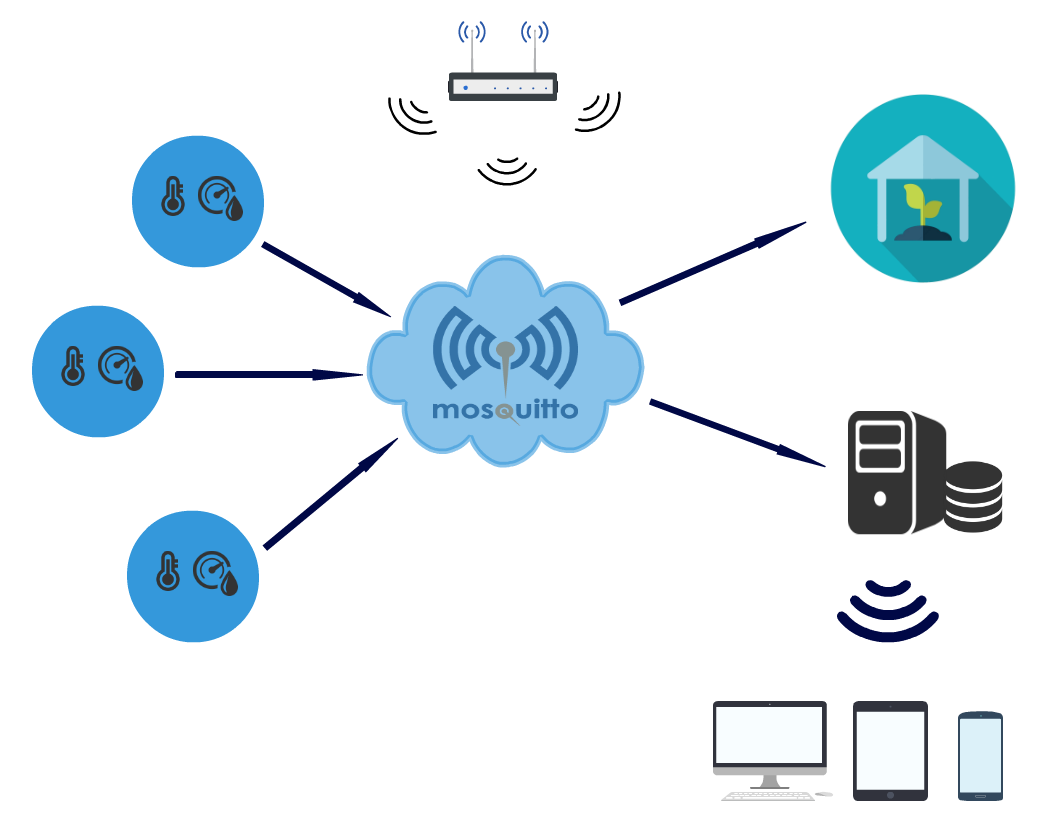
\includegraphics[scale=0.3]{./04-figuras/rede.png}
% \caption{Esquema da rede de sensores}
% \vspace{-\baselineskip}
% \fonte{Do autor}
% \label{fig:esquema-rede}
% \end{figure}

\section{Aplicação Web}
Nesta seção serão apresentados os passos seguidos no desenvolvimento da aplicação, tais como o processo de desenvolvimento de software e tecnologias empregadas.

\subsection{Processo de Desenvolvimento de \textit{Software}} 
O processo de desenvolvimento de \textit{software} utilizado foi o Iterativo e Incremental. Esse processo consiste em um ciclo onde são realizadas tentativas sucessivas de refinamento, a cada iteração são realizadas melhorias no \textit{software}.

\citeonline{bezerra2017iterativoeincremental} define o processo Iterativo e Incremental como um conjunto de ciclos, onde cada ciclo considera um subconjunto de requisitos. Uma vez que estes requisitos são implementados um novo ciclo se inicia, e com este novo ciclo um novo subconjunto de requisitos é considerado para ser desenvolvido, o que produz um novo incremento do sistema. Dessa forma, o desenvolvimento evolui em versões, ao longo da construção incremental e iterativa de novas funcionalidades até que o sistema completo esteja construído.

\begin{figure}[H]
    \centering
    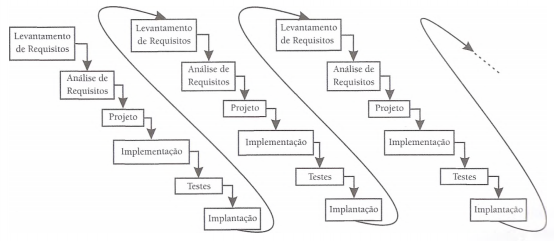
\includegraphics[scale=0.7]{04-figuras/iterativo-incremental.png}
    \caption{Etapas a serem realizadas a cada ciclo}
    \vspace{-\baselineskip}
    \fonte{\cite{bezerra2017iterativoeincremental}}
    \label{fig:iterativo-incremental}
\end{figure}

Como pode ser observado na figura \ref{fig:iterativo-incremental}, cada ciclo do processo Iterativo e Incremental é composto pelas etapas de análise e levantamento de requisitos, projeto de software, implementação, testes e implantação. \citeonline{bezerra2017iterativoeincremental} ainda afirma que a abordagem incremental estimula a participação do usuário nas etapas do desenvolvimento, o que diminui a chance de ocorrer interpretações erradas em relação aos requisitos levantados, além de também possibilitar um melhor gerenciamento em relação aos riscos do projeto.

\subsection{Levantamento e Análise de Requisitos}
O primeiro passo realizado no desenvolvimento do sistema foi o levantamento de requisitos. Este levantamento foi realizado através de reuniões juntamente ao professor responsável pelo setor de fruticultura. Durante estas reuniões foram definidas as funcionalidades que atendem às necessidades do setor. Após o levantamento ser concluído, foi feito uma análise desses requisitos juntamente ao professor orientador do trabalho, onde foi definido um escopo viável para implementar. 

\subsection{Projeto de \textit{Software}}
Para o projeto de \textit{software} foi utilizada a Linguagem de Modelagem Unificada (UML), esta linguagem permite a modelagem de sistemas através de elementos gráficos, como diagramas \cite{bezerra2017iterativoeincremental}. 

\begin{figure}[H]
    \centering
    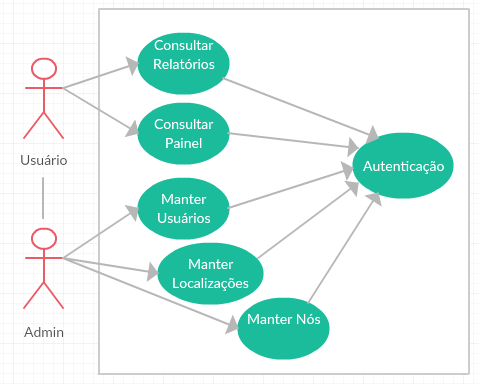
\includegraphics[scale=0.8]{04-figuras/caso_de_uso.png}
    \caption{Diagrama de caso de uso}
    \vspace{-\baselineskip}
    \fonte{Do autor}
    \label{fig:caso-de-uso}
\end{figure}

Nesta etapa foi desenvolvido o diagrama de caso de uso (figura \ref{fig:caso-de-uso}), este diagrama representa a iteração do ator (usuário) com as funcionalidades do sistema através de fluxos \cite{gomes2003casodeuso}.

Como mostra a figura \ref{fig:caso-de-uso}, o sistema conta com dois atores, que representam os
dois grupos de usuários que utilizaram o sistema. O ator "Usuário" tem acesso às funcionalidades de "Consultar Painel" e "Consultar Relatórios", já o ator "Admin", além de herdar estas funcionalidades do ator "Usuário", também possui acesso às funcionalidades de "Manter Localizações", "Manter nós" e "Manter Usuários". Todas as funcionalidades do sistema exigem que o usuário esteja autenticado. O verbo "manter", presente nas funcionalidades, representa quatro operações básicas de banco de dados, \textit{Create, Read, Update e Delete} (CRUD).

\subsection{Implementação}
A implementação do sistema foi dividida em duas partes, \textit{back-end} e \textit{front-end}. O \textit{back-end}, como o próprio nome sugere, é a parte de "trás" da aplicação. É a parte da aplicação que roda no servidor e é responsável pela implementação da regra de negócio. Já o termo \textit{front-end} se refere à parte de interface do sistema, ou seja, é a parte da aplicação que interage diretamente com o usuário.

\subsubsection{\textit{Back-end}}
O \textit{backend} foi desenvolvido utilizando NodeJS\footnote{Mais informações sobre Nodejs podem ser acessadas em: \url{https://nodejs.org/en/}}, que é um interpretador JavaScript \textit{open source} que possibilita a sua utilização como linguagem de servidor, através do \textit{framework web} AdonisJS\footnote{Mais informações sobre Adonisjs podem ser acessadas em: \url{https://adonisjs.com/}}. O desenvolvimento seguirá o padrão \textit{Model, View, Controller} (MVC).

\begin{figure}[H]
    \centering
    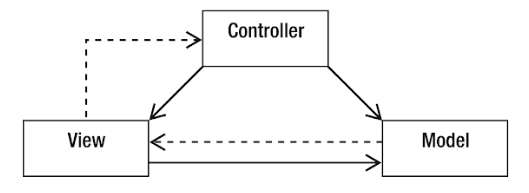
\includegraphics[scale=1]{04-figuras/mvc.png}
    \caption{Arquitetura do padrão MVC}
    \vspace{-\baselineskip}
    \fonte{\cite{dooley2011mvc}}
    \label{fig:mvc}
\end{figure}

Como podemos ver na figura \ref{fig:mvc}, o padrão MVC se divide em três camadas:
\begin{itemize}[itemsep=0em]
    \item \textit{\textbf{Controller}} (controlador): o controlador interpreta as entradas enviadas pelo usuário e as mapeia em comandos que serão enviados para o modelo e/ou para uma janela de visualização \cite{dooley2011mvc}.
    \item \textit{\textbf{Model}} (modelo): o modelo gerencia os elementos de dados, nesta camada que é realizado a comunicação com o banco de dados  \cite{dooley2011mvc}.
    \item \textit{\textbf{View}} (visão): visão é a camada responsável por apresentar os dados ao usuário \cite{dooley2011mvc}.
\end{itemize}

Como banco de dados foi escolhido o MongoDB, que é um software de banco de dados \textit{open source} orientado a documentos e multiplataforma. 
\vfill

\subsubsection{\textit{Front-end}}
O \textit{front-end} do sistema foi desenvolvido utilizando a linguagem JavaScript por meio da biblioteca ReactJS. Esta biblioteca foi desenvolvida pela equipe de desenvolvedores do Facebook e Instagram, é uma biblioteca que funciona na ideia de componentização, onde a ideia é quebrar os elementos em pequenos componentes reutilizáveis. Para desenvolvimento da interface foram empregados os conceitos de \textit{Material Design} por meio do \textit{framework} Material UI que implementa esse conceito.

\subsection{Testes e Implantação}
Nesta etapa do desenvolvimento serão realizados testes automatizados nas funcionalidades do sistema. Após testadas as funcionalidades serão efetuados testes de usabilidade da aplicação buscando um \textit{feedback} do usuário para que o sistema possa ser melhorado. Realizado os devidos testes se dará inicio a mais um ciclo de desenvolvimento, este ciclo se repetirá até que o sistema completo esteja concluído e valido para que possa ser implantado.

\section{Experimentos}
Nesta etapa serão efetuados experimentos visando verificar se o trabalho desenvolvido cumpre a proposta de trazer melhorias na produção. Serão separados dois ambientes distintos:

\begin{itemize}[itemsep=0em]
\item O primeiro ambiente estará sob as condições atuais onde o sistema nebulizador é acionado de maneira estática.
\item O segundo ambiente estará sendo controlado pelo sistema desenvolvido.
\end{itemize}

Serão colocadas mudas nos dois ambientes para que possa ser avaliado sob quais condições será obtido o melhor resultado.